\chapter{PROPOSED SOLUTION}
\label{chap:solution}
\section{Data collecting with crowd-sourcing model}
A traditional method of collecting data is to do it manually : Setting up an array of cameras at desired locations and then obtain their recordings. Those recording would later be labeled by specialists or experts and processed to form a dataset. This way of approach is expensive and requires a lot of human resources.

One other method of data collection is to implement Web crawler to pull data from the internet automatically. This method would be most useful for getting a large amount of data given a keyword. One downside is that data achieved by this method often contain considerable noise because of typos, mislabel or error. In the context of security, those data are not suitable to be used because they are incredibly diverse and do not portray the Vietnamese environment accurately. Moreover, public data used for security matter can be collected by crawler is not considerable or may insufficient.

Crowd-sourcing is also one of the effective methods of data collection which is becoming a trend in the last couple of years. The idea behind crowd-sourcing data is to build datasets with the assistance of the community. An example of this kind of model is Wikipedia\footnotetext{\url:{https://www.wikipedia.org}}
. Wikipedia is an enormous web-based, collaborative encyclopedia which has over 100,000 volunteers contributing new information to the system daily. The success of Wikipedia proves the capability of crowd-sourcing. The solution is applicable to this project due to its advantages of significant cost saving. Furthermore, appropriate datasets can be created by Vietnamese community.

However, how can people be encouraged to provide their knowledge and information? Interaction with others is proven successful in encouraging people to share.Therefore, social media has been a popular trend among Vietnamese in recent years. At the time of November 2018, the amount of people using Facebook has reached about 70 million, that accounts for almost 73\% of the population. (Figure \ref{chap3:social_media_vn}).

\begin{center}
    \begin{figure}[H]
    \centering
    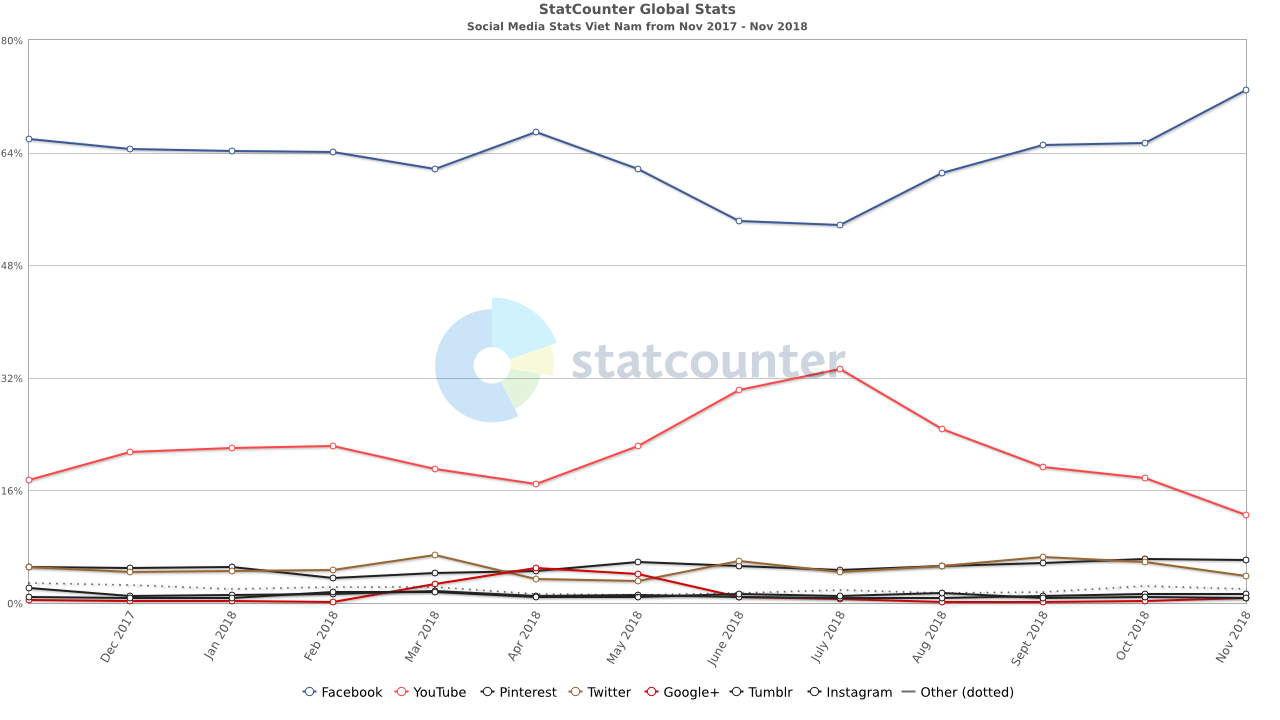
\includegraphics[width=1\columnwidth]{images/chap3/social_media_vn.png}
    \footcaption{Social media usage of Vietnamese is at all time high. Nearly 73\% of the population is using use Facebook}
    \label{chap3:social_media_vn}
    \end{figure}
\end{center}
\footnotetext{Source: \url:{http://gs.statcounter.com/social-media-stats/all/viet-nam}}
Because of mentioned factors, this thesis proposes building a \textbf{Social media website for security} where users can interact with each other, as well as provide their data to the system via posting.
\section{Extracting information from data}

\subsection{Image}

Data received by the system will include images and videos. %%Kha làm
 
There are many ways to recognize faces through APIs such as Kairos, Amazon Rekognition, Microsoft Face API, Google Cloud Vision, and IDM Watson Visual Recognition, and these are their features:
\begin{center}
	\begin{figure}[H]
		\centering
		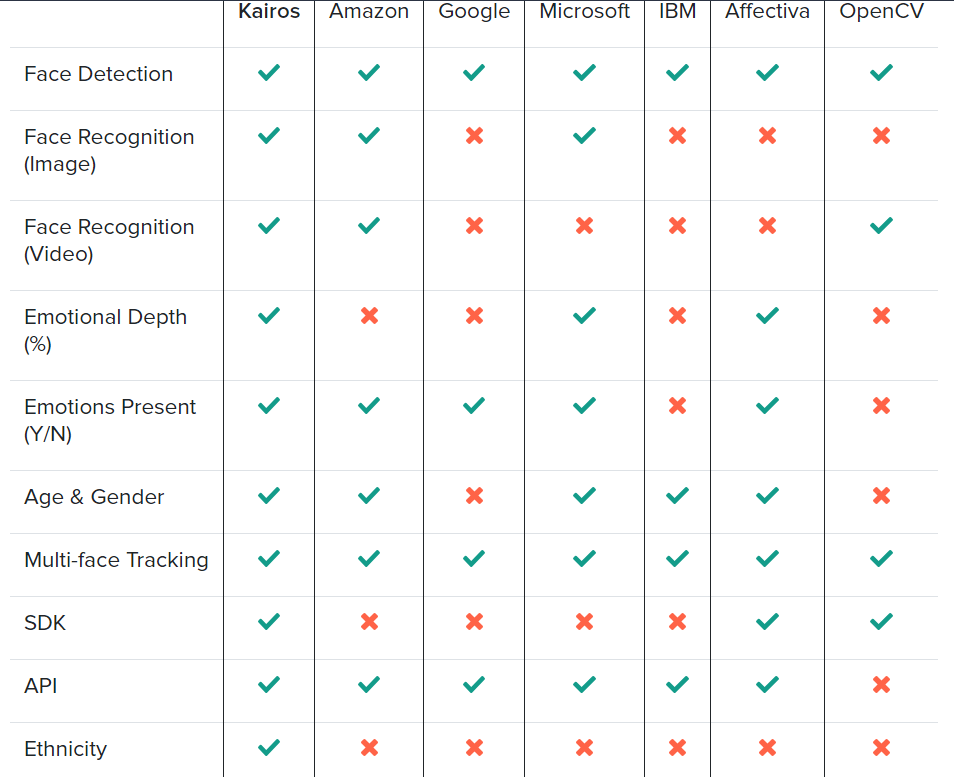
\includegraphics[width=1\columnwidth]{images/chap3/face_api.png}
		\footcaption{Feature of all recent famouse face api}
		\label{chap3:face_api_now}
	\end{figure}
\end{center}
\footnotetext{Source: \url:{https://www.kairos.com/blog/face-recognition-kairos-vs-microsoft-vs-google-vs-amazon-vs-opencv}}
\begin{itemize}
	\item  Kairos: offers a wide variety of image recognition solutions through their API. Their API endpoints include identifying gender, age, emotional depth, facial recognition in both photo and video, and more.
	\item Amazon Rekognition: This facial recognition API is fully integrated into the Amazon Web Service ecosystem. Using this API will make it easy to build applications that make use of other AWS products.
	\item Google Cloud Vision: By being integrated into the Google Cloud Platform, this API will be a breeze to integrate into applications that are already using other Google Cloud Platform products and services.
\end{itemize}

However, with the limitations of the thesis and the applicability to fulfill demands of this research, Microsoft Face API is choosen. There are many advantage of Microsoft Face API such as large amount of user identification, high accuracy and lower cost of usage than the whole API remaining at the time of the investigation


\subsection{Video}
For the video analyzing problem, this thesis proposes using a video classification model to find out if there are suspicious behaviors within a video. This model processes videos by passing frames through a Convolutional Neural Network to extract features, then pass the output to a Recurrent Neural Network using LSTM cells, similar to the approach of \cite{DBLP:journals/corr/DonahueHGRVSD14} and \cite{}. This model was trained and test using UCF-101 dataset\footnotetext{Source: url:{http://crcv.ucf.edu/data/UCF101.php}} - A standard dataset commonly used for benchmarking action recognition models - and achieved a moderate result.
\subsection{Proposed Architecture}
\subsubsection{CNN architecture for feature extraction}
In \cite{DBLP:journals/corr/ZhouKLOT14}, the authors suggest that pretrained CNNs are incredibly effective in extracting feature for other classification tasks.
For the CNN layer of the proposal model, a VGG16 \cite{DBLP:journals/corr/SimonyanZ14a} architecture pretrained on ImageNet \footnotetext{Source: \url:{http://www.image-net.org/challenges/LSVRC/}} is chosen to extract features from video frames. Figure \ref{chap3:vgg16_architecture} shows the architecture of this model. Input of VGG16 is an 224x224x3 RGB image. The image is then pass through a stack of convolutional layers. All of hidden layers are equipped with a ReLU.  
\begin{center}
    \begin{figure}[H]
    \centering
    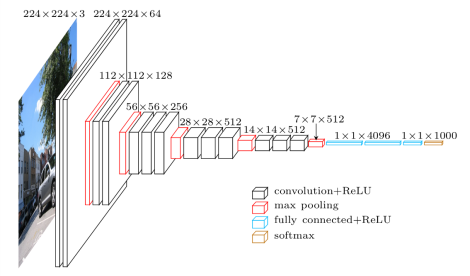
\includegraphics[width=1\columnwidth]{images/chap3/vgg16_architecture.png}
    \footcaption{}
    \label{chap3:vgg16_architecture}
    \end{figure}
\end{center}
\footnotetext{Source: \url:{https://blog.heuritech.com/2016/02/29/a-brief-report-of-the-heuritech-deep-learning-meetup-5/}}
\subsubsection{LSTM for sequence learning}
Output of VGG16 is passed through LSTM cells for prediction.
Lost function
\subsection{Dataset}
\subsection{Evaluating}
\subsubsection{Preprocessing}
\subsubsection{Hyperparameter}
\subsubsection{Training method}
\subsection{Result}





